
%% bare_conf.tex
%% V1.4b
%% 2015/08/26
%% by Michael Shell
%% See:
%% http://www.michaelshell.org/
%% for current contact information.
%%
%% This is a skeleton file demonstrating the use of IEEEtran.cls
%% (requires IEEEtran.cls version 1.8b or later) with an IEEE
%% conference paper.
%%
%% Support sites:
%% http://www.michaelshell.org/tex/ieeetran/
%% http://www.ctan.org/pkg/ieeetran
%% and
%% http://www.ieee.org/

%%*************************************************************************
%% Legal Notice:
%% This code is offered as-is without any warranty either expressed or
%% implied; without even the implied warranty of MERCHANTABILITY or
%% FITNESS FOR A PARTICULAR PURPOSE! 
%% User assumes all risk.
%% In no event shall the IEEE or any contributor to this code be liable for
%% any damages or losses, including, but not limited to, incidental,
%% consequential, or any other damages, resulting from the use or misuse
%% of any information contained here.
%%
%% All comments are the opinions of their respective authors and are not
%% necessarily endorsed by the IEEE.
%%
%% This work is distributed under the LaTeX Project Public License (LPPL)
%% ( http://www.latex-project.org/ ) version 1.3, and may be freely used,
%% distributed and modified. A copy of the LPPL, version 1.3, is included
%% in the base LaTeX documentation of all distributions of LaTeX released
%% 2003/12/01 or later.
%% Retain all contribution notices and credits.
%% ** Modified files should be clearly indicated as such, including  **
%% ** renaming them and changing author support contact information. **
%%*************************************************************************


% *** Authors should verify (and, if needed, correct) their LaTeX system  ***
% *** with the testflow diagnostic prior to trusting their LaTeX platform ***
% *** with production work. The IEEE's font choices and paper sizes can   ***
% *** trigger bugs that do not appear when using other class files.       ***                          ***
% The testflow support page is at:
% http://www.michaelshell.org/tex/testflow/



\documentclass[conference]{IEEEtran}
% Some Computer Society conferences also require the compsoc mode option,
% but others use the standard conference format.
%
% If IEEEtran.cls has not been installed into the LaTeX system files,
% manually specify the path to it like:
% \documentclass[conference]{../sty/IEEEtran}





% Some very useful LaTeX packages include:
% (uncomment the ones you want to load)


% *** MISC UTILITY PACKAGES ***
%
%\usepackage{ifpdf}
% Heiko Oberdiek's ifpdf.sty is very useful if you need conditional
% compilation based on whether the output is pdf or dvi.
% usage:
% \ifpdf
%   % pdf code
% \else
%   % dvi code
% \fi
% The latest version of ifpdf.sty can be obtained from:
% http://www.ctan.org/pkg/ifpdf
% Also, note that IEEEtran.cls V1.7 and later provides a builtin
% \ifCLASSINFOpdf conditional that works the same way.
% When switching from latex to pdflatex and vice-versa, the compiler may
% have to be run twice to clear warning/error messages.






% *** CITATION PACKAGES ***
%
%\usepackage{cite}
% cite.sty was written by Donald Arseneau
% V1.6 and later of IEEEtran pre-defines the format of the cite.sty package
% \cite{} output to follow that of the IEEE. Loading the cite package will
% result in citation numbers being automatically sorted and properly
% "compressed/ranged". e.g., [1], [9], [2], [7], [5], [6] without using
% cite.sty will become [1], [2], [5]--[7], [9] using cite.sty. cite.sty's
% \cite will automatically add leading space, if needed. Use cite.sty's
% noadjust option (cite.sty V3.8 and later) if you want to turn this off
% such as if a citation ever needs to be enclosed in parenthesis.
% cite.sty is already installed on most LaTeX systems. Be sure and use
% version 5.0 (2009-03-20) and later if using hyperref.sty.
% The latest version can be obtained at:
% http://www.ctan.org/pkg/cite
% The documentation is contained in the cite.sty file itself.

\usepackage{graphicx}


% *** GRAPHICS RELATED PACKAGES ***
%
%\ifCLASSINFOpdf
  %\usepackage[pdftex]{graphicx}
  % declare the path(s) where your graphic files are
  % \graphicspath{{../pdf/}{../jpeg/}}
  % and their extensions so you won't have to specify these with
  % every instance of \includegraphics
  % \DeclareGraphicsExtensions{.pdf,.jpeg,.png}
%\else
  % or other class option (dvipsone, dvipdf, if not using dvips). graphicx
  % will default to the driver specified in the system graphics.cfg if no
  % driver is specified.
  % \usepackage[dvips]{graphicx}
  % declare the path(s) where your graphic files are
  % \graphicspath{{../eps/}}
  % and their extensions so you won't have to specify these with
  % every instance of \includegraphics
  % \DeclareGraphicsExtensions{.eps}
%\fi
% graphicx was written by David Carlisle and Sebastian Rahtz. It is
% required if you want graphics, photos, etc. graphicx.sty is already
% installed on most LaTeX systems. The latest version and documentation
% can be obtained at: 
% http://www.ctan.org/pkg/graphicx
% Another good source of documentation is "Using Imported Graphics in
% LaTeX2e" by Keith Reckdahl which can be found at:
% http://www.ctan.org/pkg/epslatex
%
% latex, and pdflatex in dvi mode, support graphics in encapsulated
% postscript (.eps) format. pdflatex in pdf mode supports graphics
% in .pdf, .jpeg, .png and .mps (metapost) formats. Users should ensure
% that all non-photo figures use a vector format (.eps, .pdf, .mps) and
% not a bitmapped formats (.jpeg, .png). The IEEE frowns on bitmapped formats
% which can result in "jaggedy"/blurry rendering of lines and letters as
% well as large increases in file sizes.
%
% You can find documentation about the pdfTeX application at:
% http://www.tug.org/applications/pdftex





% *** MATH PACKAGES ***
%
\usepackage{amsmath}
% A popular package from the American Mathematical Society that provides
% many useful and powerful commands for dealing with mathematics.
%
% Note that the amsmath package sets \interdisplaylinepenalty to 10000
% thus preventing page breaks from occurring within multiline equations. Use:
%\interdisplaylinepenalty=2500
% after loading amsmath to restore such page breaks as IEEEtran.cls normally
% does. amsmath.sty is already installed on most LaTeX systems. The latest
% version and documentation can be obtained at:
% http://www.ctan.org/pkg/amsmath


\usepackage{mathrsfs}



% *** SPECIALIZED LIST PACKAGES ***
%
%\usepackage{algorithmic}
% algorithmic.sty was written by Peter Williams and Rogerio Brito.
% This package provides an algorithmic environment fo describing algorithms.
% You can use the algorithmic environment in-text or within a figure
% environment to provide for a floating algorithm. Do NOT use the algorithm
% floating environment provided by algorithm.sty (by the same authors) or
% algorithm2e.sty (by Christophe Fiorio) as the IEEE does not use dedicated
% algorithm float types and packages that provide these will not provide
% correct IEEE style captions. The latest version and documentation of
% algorithmic.sty can be obtained at:
% http://www.ctan.org/pkg/algorithms
% Also of interest may be the (relatively newer and more customizable)
% algorithmicx.sty package by Szasz Janos:
% http://www.ctan.org/pkg/algorithmicx




% *** ALIGNMENT PACKAGES ***
%
%\usepackage{array}
% Frank Mittelbach's and David Carlisle's array.sty patches and improves
% the standard LaTeX2e array and tabular environments to provide better
% appearance and additional user controls. As the default LaTeX2e table
% generation code is lacking to the point of almost being broken with
% respect to the quality of the end results, all users are strongly
% advised to use an enhanced (at the very least that provided by array.sty)
% set of table tools. array.sty is already installed on most systems. The
% latest version and documentation can be obtained at:
% http://www.ctan.org/pkg/array


% IEEEtran contains the IEEEeqnarray family of commands that can be used to
% generate multiline equations as well as matrices, tables, etc., of high
% quality.




% *** SUBFIGURE PACKAGES ***
%\ifCLASSOPTIONcompsoc
%  \usepackage[caption=false,font=normalsize,labelfont=sf,textfont=sf]{subfig}
%\else
%  \usepackage[caption=false,font=footnotesize]{subfig}
%\fi
% subfig.sty, written by Steven Douglas Cochran, is the modern replacement
% for subfigure.sty, the latter of which is no longer maintained and is
% incompatible with some LaTeX packages including fixltx2e. However,
% subfig.sty requires and automatically loads Axel Sommerfeldt's caption.sty
% which will override IEEEtran.cls' handling of captions and this will result
% in non-IEEE style figure/table captions. To prevent this problem, be sure
% and invoke subfig.sty's "caption=false" package option (available since
% subfig.sty version 1.3, 2005/06/28) as this is will preserve IEEEtran.cls
% handling of captions.
% Note that the Computer Society format requires a larger sans serif font
% than the serif footnote size font used in traditional IEEE formatting
% and thus the need to invoke different subfig.sty package options depending
% on whether compsoc mode has been enabled.
%
% The latest version and documentation of subfig.sty can be obtained at:
% http://www.ctan.org/pkg/subfig




% *** FLOAT PACKAGES ***
%
%\usepackage{fixltx2e}
% fixltx2e, the successor to the earlier fix2col.sty, was written by
% Frank Mittelbach and David Carlisle. This package corrects a few problems
% in the LaTeX2e kernel, the most notable of which is that in current
% LaTeX2e releases, the ordering of single and double column floats is not
% guaranteed to be preserved. Thus, an unpatched LaTeX2e can allow a
% single column figure to be placed prior to an earlier double column
% figure.
% Be aware that LaTeX2e kernels dated 2015 and later have fixltx2e.sty's
% corrections already built into the system in which case a warning will
% be issued if an attempt is made to load fixltx2e.sty as it is no longer
% needed.
% The latest version and documentation can be found at:
% http://www.ctan.org/pkg/fixltx2e


%\usepackage{stfloats}
% stfloats.sty was written by Sigitas Tolusis. This package gives LaTeX2e
% the ability to do double column floats at the bottom of the page as well
% as the top. (e.g., "\begin{figure*}[!b]" is not normally possible in
% LaTeX2e). It also provides a command:
%\fnbelowfloat
% to enable the placement of footnotes below bottom floats (the standard
% LaTeX2e kernel puts them above bottom floats). This is an invasive package
% which rewrites many portions of the LaTeX2e float routines. It may not work
% with other packages that modify the LaTeX2e float routines. The latest
% version and documentation can be obtained at:
% http://www.ctan.org/pkg/stfloats
% Do not use the stfloats baselinefloat ability as the IEEE does not allow
% \baselineskip to stretch. Authors submitting work to the IEEE should note
% that the IEEE rarely uses double column equations and that authors should try
% to avoid such use. Do not be tempted to use the cuted.sty or midfloat.sty
% packages (also by Sigitas Tolusis) as the IEEE does not format its papers in
% such ways.
% Do not attempt to use stfloats with fixltx2e as they are incompatible.
% Instead, use Morten Hogholm'a dblfloatfix which combines the features
% of both fixltx2e and stfloats:
%
% \usepackage{dblfloatfix}
% The latest version can be found at:
% http://www.ctan.org/pkg/dblfloatfix




% *** PDF, URL AND HYPERLINK PACKAGES ***
%
%\usepackage{url}
% url.sty was written by Donald Arseneau. It provides better support for
% handling and breaking URLs. url.sty is already installed on most LaTeX
% systems. The latest version and documentation can be obtained at:
% http://www.ctan.org/pkg/url
% Basically, \url{my_url_here}.




% *** Do not adjust lengths that control margins, column widths, etc. ***
% *** Do not use packages that alter fonts (such as pslatex).         ***
% There should be no need to do such things with IEEEtran.cls V1.6 and later.
% (Unless specifically asked to do so by the journal or conference you plan
% to submit to, of course. )

% *** Pseudocode PACKAGES ***
\usepackage{amsmath}
\usepackage{algorithm}
\usepackage{varwidth}
\usepackage[noend]{algpseudocode}
\makeatletter
\def\BState{\State\hskip-\ALG@thistlm}
\makeatother


\newcommand\NB[1]{$\spadesuit$\footnote{NB: #1}}
% reference package for bibtex

%\usepackage{biblatex}
%\addbibresource{mybibliography.bib}

%\usepackage[
%backend=biber,
%style=numeric,
%sorting=ynt
%]{biblatex}

%\addbibresource{mybibliography.bib}


% correct bad hyphenation here
\hyphenation{op-tical net-works semi-conduc-tor}


\begin{document}
%
% paper title
% Titles are generally capitalized except for words such as a, an, and, as,
% at, but, by, for, in, nor, of, on, or, the, to and up, which are usually
% not capitalized unless they are the first or last word of the title.
% Linebreaks \\ can be used within to get better formatting as desired.
% Do not put math or special symbols in the title.
\title{Using Hidden Markov Models to Improve Autonomous Vehicle Decision Making - Problem Formulation}


% author names and affiliations
% use a multiple column layout for up to three different
% affiliations
\author{\IEEEauthorblockN{Rahul Peddi}
\IEEEauthorblockA{Systems and Information Engineering\\
University of Virginia\\
Charlottesville, Virginia\\
Email: rp3cy@virginia.edu}}

% conference papers do not typically use \thanks and this command
% is locked out in conference mode. If really needed, such as for
% the acknowledgment of grants, issue a \IEEEoverridecommandlockouts
% after \documentclass

% for over three affiliations, or if they all won't fit within the width
% of the page, use this alternative format:
% 
%\author{\IEEEauthorblockN{Michael Shell\IEEEauthorrefmark{1},
%Homer Simpson\IEEEauthorrefmark{2},
%James Kirk\IEEEauthorrefmark{3}, 
%Montgomery Scott\IEEEauthorrefmark{3} and
%Eldon Tyrell\IEEEauthorrefmark{4}}
%\IEEEauthorblockA{\IEEEauthorrefmark{1}School of Electrical and Computer Engineering\\
%Georgia Institute of Technology,
%Atlanta, Georgia 30332--0250\\ Email: see http://www.michaelshell.org/contact.html}
%\IEEEauthorblockA{\IEEEauthorrefmark{2}Twentieth Century Fox, Springfield, USA\\
%Email: homer@thesimpsons.com}
%\IEEEauthorblockA{\IEEEauthorrefmark{3}Starfleet Academy, San Francisco, California 96678-2391\\
%Telephone: (800) 555--1212, Fax: (888) 555--1212}
%\IEEEauthorblockA{\IEEEauthorrefmark{4}Tyrell Inc., 123 Replicant Street, Los Angeles, California 90210--4321}}




% use for special paper notices
%\IEEEspecialpapernotice{(Invited Paper)}




% make the title area
\maketitle

% As a general rule, do not put math, special symbols or citations
% in the abstract
\begin{abstract}
\end{abstract}

% no keywords




% For peer review papers, you can put extra information on the cover
% page as needed:
% \ifCLASSOPTIONpeerreview
% \begin{center} \bfseries EDICS Category: 3-BBND \end{center}
% \fi
%
% For peerreview papers, this IEEEtran command inserts a page break and
% creates the second title. It will be ignored for other modes.
\IEEEpeerreviewmaketitle



\section{Introduction}
% no \IEEEPARstart
    Over the last few years, semi-autonomous and autonomous vehicles have become increasingly popular, but they have not replaced traditional vehicles entirely just yet. This leads to a hybrid environment; one that features vehicles of all levels of autonomy. Many of these vehicles to be equipped with some form of adaptive cruise control (ACC) or advance driver assistance systems (ADAS), both of which help the driver make safe decisions while operating the vehicle. These types of systems are forms of human-robot interaction. ACC performs actions autonomously and works at the command of a human who determines a target velocity and a safe following distance. ADAS, on the contrary, acts as an information system for human drivers. These systems, however, are limited in their capabilities as they require constant monitoring from the driver and are unable to predict if the driver will enter a dangerous situation in the future. In addition, these systems can fail to guarantee safety in rapidly transitioning environments.
    
    One such example of an environment in which dangers arise rapidly are highways. Highways are often comprised of multiple lanes and many drivers performing different behaviors including lane changes, merges, passing, and reacting to other vehicles. In addition, highways involve traveling at very high velocities, which increase the likelihood that a dangerous situation will arise. \NB{I would keep this more general. We don't want to have a paper about highway safety. The highway should be an example}
    
    Because these dangerous situations can occur so rapidly \NB{need citation here}, there is a need to increase the ability to guarantee safety when developing new systems \NB{what do you mean with new systems?} for human drivers. This can be done by increasing the ability to predict and adapt to what will happen in the future. A simple depiction of a danger situation is shown in Fig. \ref{fig:hiway}. \NB{figure needs improvements}

\begin{figure}[ht]
    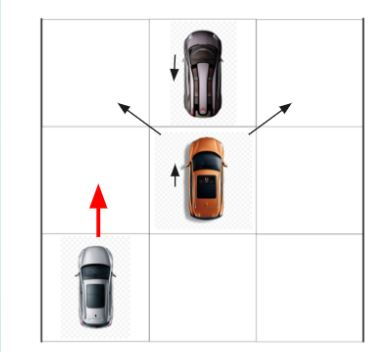
\includegraphics[width=0.5\textwidth]{highwaysit.JPG}
    \caption{Potentially dangerous highway situation. The vehicle in the center of the grid is the host vehicle, and the vehicle in front is driving much slower, while the vehicle to the right is approaching very rapidly. It would be safe in the instant to pass on the left, but that leaves the possibility that a dangerous situation will occur very soon.}
    \label{fig:hiway}
\end{figure}
    
    In terms of the adaptation, the human driver does control the vehicle, but it is important to have to ability to intervene and adjust the driver's actions as a dangerous situation arises. In this work, we aim to provide
    \begin{itemize}
    \item{a prediction method that can effectively and efficiently estimate the future positions of surrounding agents}
    \item{an adaptive framework that determines the adjustment and severity of such adjustment that should be made at any point in time}
    \end{itemize}
  
  \NB{we should briefly mention how we solve these problems here}  
    The rest of this paper is organized as follows: in Section II, we discuss related work, and in Section III, we formally define the problem. The method to predict future behaviors and positions of other vehicles are presented in Section IV. We demonstrate our results with simulations and experiments in Sections V and VI, respectively.Lastly, we discuss our conclusions and discuss future work in Section VII.

    
% You must have at least 2 lines in the paragraph with the drop letter
% (should never be an issue)

\section{Related Work}

%    This work is tuned a relatively specific situation; one where the host vehicle is driving in the middle lane of a three-lane highway. This was chosen in order to account for a large action space. In this case, there are three possible actions the host vehicle could take, and each of these actions is evaluated for safety. The action space is defined such that it only looks at the immediately adjacent lanes. For example, if the vehicle is in the left lane, the action space consists of forward, and move right. In this case, only those two actions are evaluated for safety at a future time step.
    
    
%    A Hidden Markov Model is a type of Markov Model, where the states are hidden. A Markov Model examines states and transitions to and from these states. An HMM operates on the assumption that we don't directly know what the state is, but we are able to make observations that can tell us valuable information about the current state. Hidden Markov Models have been used for many human-robot interaction applications \cite{li2016modeling}, including but not limited to speech recognition, motion recognition, and biological analyses \cite{yoon2009hidden}.
    
%    In addition to the host vehicle at the center of the road, there are two additional vehicles; one passing on the left lane, and a slowed vehicle ahead in the center lane, as shown in Figure \ref{fig:actionspace}.
    
%    The HMM was performed on the blue vehicle to the left (the purple vehicle is a representation of the estimate), from the perspective of the black vehicle, the host vehicle. The testing was done such that only one vehicle was able to make estimations, but in a truly hybrid environment, multiple vehicles will this technique will improve the ability for multiple vehicles to collaborate.
    
\section{Problem Formulation}
 
    In this work, we are interested in developing a technique that assists a human-operated vehicle in predicting and adapting to the future states of neighboring vehicles in a dynamic environment. The problem can be formally laid out as follows:
    
    A manned vehicle is moving in an environment in the presence of stationary obstacles and other vehicles. The goal ensure safe operation in cluttered environments.
    
    %To determine a policy that predicts the future states of neighboring vehicles and the likelihood that those states will occur, while also determining the risk - wasn't sure where exactly this should go.
    
    
    
    \textbf{Problem 1: \textit{Predicting the future states of neighboring vehicles}:}
	Given a dynamic environment with multiple vehicles, a manned vehicle $\mathcal{R}$, has the objective operative in a safe manner. The aim is to find a policy that predicts the future states of neighboring vehicles and stationary obstacles within a certain sensing range of $\delta$. The neighboring vehicles are identified in 1.
	
	\begin{equation}
	    i\in S \text{ if } \rVert x_{i}-x_{\mathcal{R}}\rVert \leq \delta 
	\end{equation}
	
	where $i$ represents a single vehicle in $S$, the set of all neighboring vehicles. The condition indicates that this vehicle, $i$, has a position, $x_{i}$, within the sensing range of the user's position at $x_{\mathcal{R}}$. The future states of the neighboring vehicle $i$ should range up to time horizon $T$, such that a predicted state is returned for each future time-step up to this horizon: 
	
	\begin{equation}
    	    x_{i,t\rightarrow T} = \{x_{i,t}, x_{i,t+1}, x_{i,t+1}, ..., x_{i,t+T}\}
	\end{equation}
	
	In addition to calculating these future states, it is imperative that the accuracy of these future positions is known. As a result the probability that each of the future positions is correct should be determined:
	
	\begin{equation}
    	    P_{x_{i,t\rightarrow T}} = \{P_{x_{i,t}}, P_{x_{i,t+1}}, P_{x_{i,t+2}}, ..., P_{x_{i,t+T}}\}
	\end{equation}
	
	
	\textbf{Problem 2: \textit{Adapting and Assisting In Dangerous Situations}:} Given the future states of $i$ and the likelihood of each state $x_{i,t\rightarrow T}$, we want to find a policy that adjusts the input,$u_{\alpha}$ provided to vehicle $\mathcal{R}$
	
\section{Proposed Method}
\subsection{Intent and Behavior Prediction}
The intent inference model is based on a Hidden Markov Model (HMM). In the implementation outlined in this work, the observations are\\

\begin{varwidth}{\textwidth}
\begin{enumerate}
  \item Speeding Up
  \item Slowing Down
  \item Maintaining
\end{enumerate}
\end{varwidth}\\
\NB{what about left right turns?}

The states are the velocities of the moving vehicle to the left of the host vehicle, and the transition and observation probabilities are generated by using the probability model below.
\begin{equation}
P(X, O \mid \mu) = \prod_{t=1}^{N} a[x_{t-1},x_{t}]b[o_{t},x_{t}]
\end{equation}

$X$ represents the sequence of states and $O$ represents the sequence of observations, and $A$ and $B$ represent the transition and observation probabilities, respectively. 

This procedure \NB{what procedure?} generates the transition probabilities that reflected\NB{why past?} the training set. The training set is of a finite length and both the velocities and the sequence of observations are recorded. The transition matrix is built in such a manner that at any velocity, the most likely following velocity can be determined \NB{how? you are not showing how this is computed}. For example, in a training set where the system measures 20 m/s in ten different instances, and in 6 of those instances the velocity jumps to 22 m/s, in 3 of them, the velocity remains at 20 m/s and in the final instance the velocity dips to 19 m/s, the transition matrix will return a 60\% chance that the following velocity is going to be 22 m/s \NB{table this more than using text}. It is possible, however, that the probabilities are equal for multiple values \NB{...and what? This sentence is incomplete. The reviewer here will be left wondering what happens if tehy have teh same prob}. The emission probability matrix illustrates whether the following velocity should be higher, lower, or the same as the current velocity. This serves to help accurately determine the expected behavior and velocity in future steps. For example, if a driver determines they are driving too fast, it's likely that they'll slow down and vice-versa. A diagram of the Hidden Markov Model is depicted in Fig.\ref{fig:hmmdiag} \NB{explain what you are showing in the diagram.}

\begin{figure}[ht]
    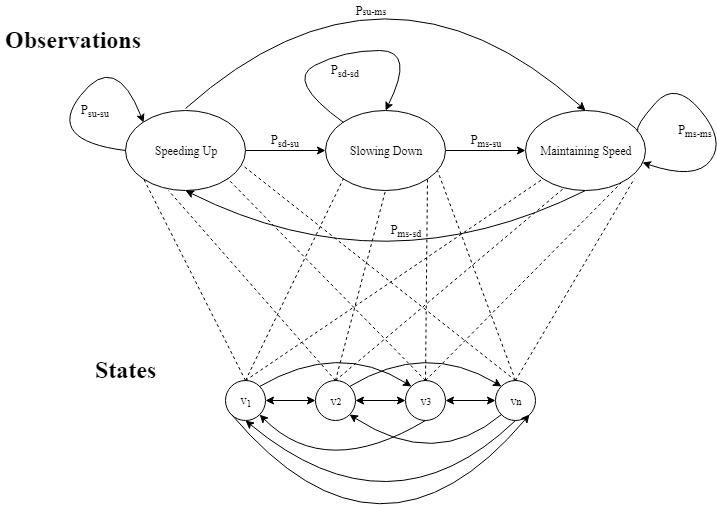
\includegraphics[width=0.5\textwidth]{hmmdiag.jpg}
    \caption{This is a visual depiction of the model used to train the prediction for future velocity states based on the observations of speeding up, slowing down, or maintaining speed.}
    \label{fig:hmmdiag}
\end{figure}

In addition to velocities, this same method is used after a certain distance behind a slower-moving vehicle to determine the behavior in that situation \NB{what nehavior, not clear}. This, in our example, is the three lanes \NB{???}. The vehicle can remain in its own lane and slow down to match, or traverse to any available adjacent lane. This model is trained similarly, where the lane the vehicle is in is the observation, and the distance after which an action occurred is the state. For both velocity and behavior HMM's, three different models were built \NB{this is not a good information to provide here. We need to be more general and show how to generate models based on training data.}; one with a fast driver, on with a medium speed driver, another with a slow driver, and conservative, medium, and aggressive lane changers; as in the distance between vehicle and obstacle decrease as aggressiveness increases.\NB{this last sentence should be moved to the simualtion section}

The purpose of the HMM is to use it to predict future states \NB{this sentence should be placed before. The sentence is contorted, simply say that the HMM is used to predict the surrounding vehicles future states and their likelihood}. In order to perform this prediction, first, observations and their matching states are compared with those of the three pre-trained models \NB{how do we so this comparison. We need to be formal here}. These models are validated using a Matlab simulation, which is shown in Fig.\ref{fig:trainset} \NB{simulations go in the simulation section}

\begin{figure}[ht]
    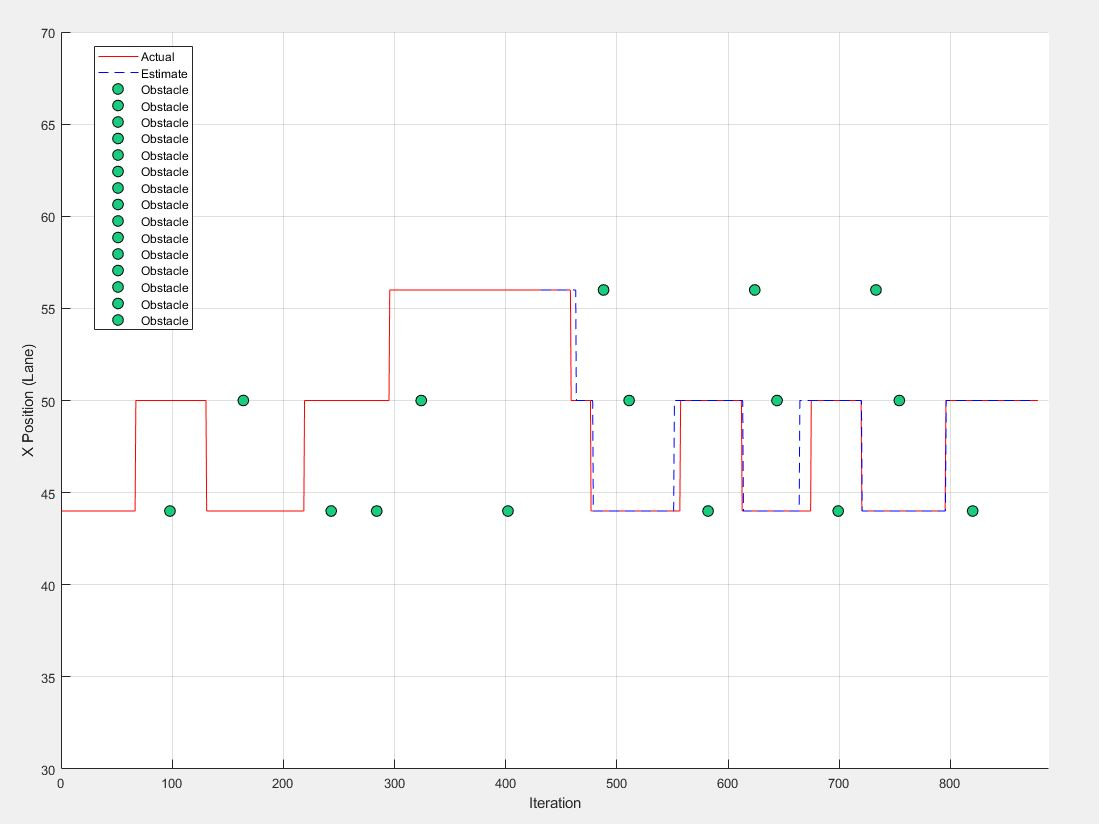
\includegraphics[width=0.5\textwidth]{trainset.JPG}
    \caption{This figure shows a period in which training occurs (prior to the appearance of the dashed line), and it also depicts an estimate, which accurately predicts what the actual vehicle does.}
    \label{fig:trainset}
\end{figure}


The best match is found using

\begin{equation}
    min dist math
\end{equation}

Once the appropriate transition and emission matrices are identified, the following maximization function is used to predict the following velocity \NB{not following, heere it looks liek you are showing in the text the following velocity. use next instead. We need to generalize that we are predicting next states which include both velocity and position}

\begin{equation}
     K_{2}\lbrack j \rbrack \gets arg \max\limits_{j}(K_{1} \lbrack j \rbrack \cdot A_{kj})
\end{equation}

This procedure gives an accurate idea of what the vehicle is going to do next. Using that, we are able to use its future position to assess possible dangers in the future.

\subsection{Risk Assessment}

The risk is calculated as a function of distance between future steps of each vehicle. This includes our vehicle, assuming the driver continues his current action \NB{not clear. Please exaplin clearly what you mean here}. A pictorial representation of this is taken from our MATLAB simulation and shown in Fig.\ref{fig:riskway}.\NB{simulations should not appear here}

\begin{figure}[ht]
    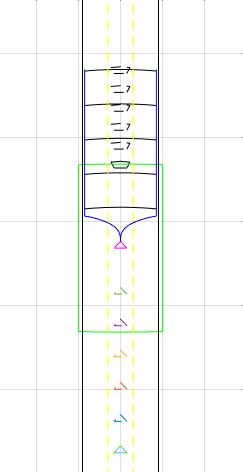
\includegraphics[height = 250,width=0.5\textwidth]{lanesandrisk.jpg}
    \caption{Future position estimates of other vehicles. The vehicle in the center is the host vehicle, in which our reachable location in 5 future time-steps are indicated by the path lines. The dotted vehicles are future estimates, and the solid lined vehicles are current locations.}
    \label{fig:riskway}
\end{figure}
The distance from each of our reachable lines at time-steps $t+1 \to t+5$ is measured and used to calculate the risk in future time-steps.

The number of future steps for which action will be taken is a user parameter. A very conservative driver could select five future time-steps, whereas an aggressive driver would select one future time-step for autonomous intervention and correction \NB{when descriving this, let's avoid to use numbers. We need to keep the theory more general. We should simply states that we are predicting N future steps ahead, or over a finite horizon of N steps}. If the user selects five time-steps as a baseline, and the system detects an unexpected peak in risk in any of the lower time-steps, action will still take place. Mathematically, the risk, $\rho$, is the inverse of the distance between two predictions,

\begin{equation}
\rho = k_{sc}\frac{1}{\Delta d},
\end{equation}

where $k_{sc}$ is a scaling constant that sets $0 \leq \rho \leq 10$ \NB{how is this possible? the equation and explanation are incorrect. Also, again, do not put absolute numbers here. We need to have general approaches}. In our work, we set three time-steps as the user parameter for risk assessment.

\subsection{Assistive Autonomous Control}

Given the range for $\rho$, a quadratic polynomial was set up in order to assign levels of autonomy, $u_{\alpha}$, to levels of risk, \NB{This needs to be revised. How did you find this. What are these numbers? We need to discuss the procedure. I need more information here. The math that you have presented so far don't make sense.}
\begin{equation}
u_{\alpha} = -0.0103\rho^{2} + 0.1989\rho + 0.0214
\end{equation}

Human control, $u_{h}$, which comprised of the rest of the control input is found using $1-u_{\alpha}$. The control of velocity is adjusted when the risk surpasses a certain threshold, $\lambda_{r}$, but minimum impact is made on the driver's intentions. This is done by calculating a $v_{max}$ and $v_{min}$ that minimize the risk. Because the risk is a function of distance, these values are set as a static distance, $\delta$ from potential obstacles on either side. In Fig.\ref{fig:vehiclepos}. \NB{no simulations here. Simulations should be presented in the simulation section}
\begin{figure}[ht]
    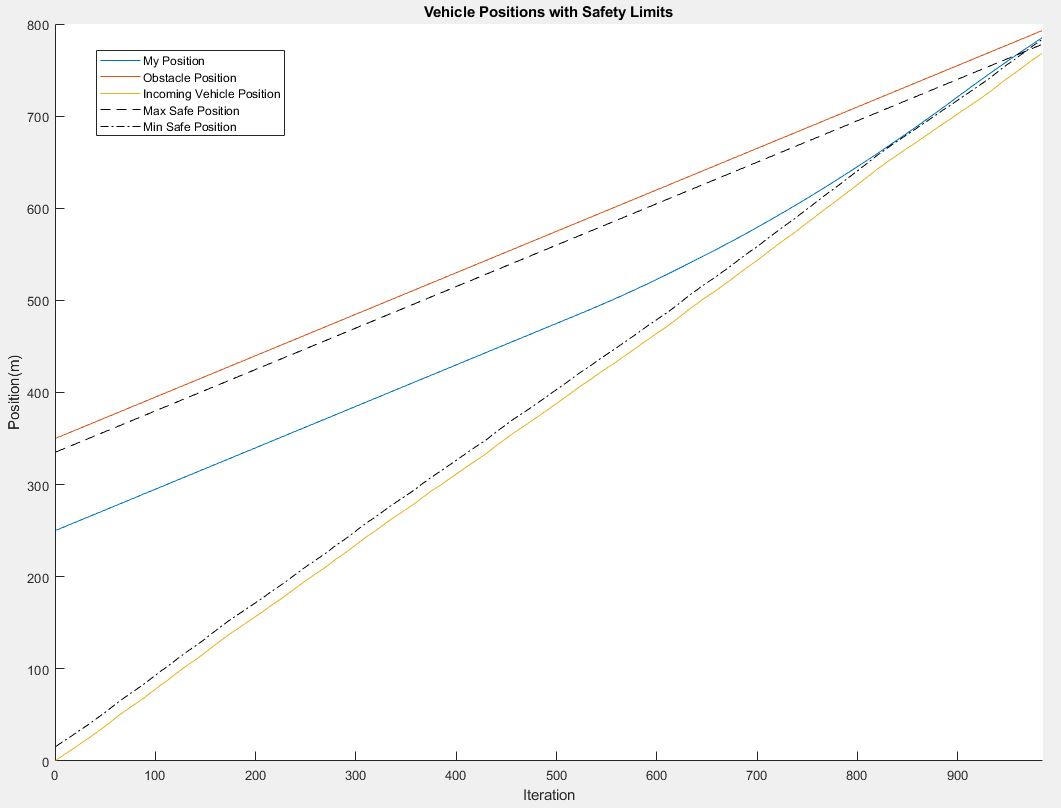
\includegraphics[width=0.5\textwidth]{vehiclepos.JPG}
    \caption{The dotted black lines represent positions that are associated with $v_{min}$ and $v_{max}$. The vehicle is minimally adjusted until the vehicle's position begins to violate either of these lines, after which point $u_{\alpha}$ increases to 1, and full control is assumed.}
    \label{fig:vehiclepos}
\end{figure}

As levels of autonomy exceed 0.5, the system begins to adjust the human's actions. This adjustment, however, is limited by $\lambda_{D}$. This is because an integral part of this system is that it is assistive, rather than fully autonomous. As $u_{\alpha}$ increases to 1.0, $\lambda_{d}$ approaches infinity, as in the limit on deviation no longer exists. This is set in order to guarantee safety in the unexpectedly dangerous situations.

\NB{the approach needs to be rewritten.}


\section{Simulations}
The simulations for this work primarily occurred in Matlab. Different case-studies were performed to indicate the ability of this system to perform under varying conditions. The first case study entails a simple response to a minimally dangerous situation, the second case study involves a more complicated situation, where a safe option is clearly available. In the third case study, we examine a situation where a clearly safe option is not present, and risk is still minimized.
\subsection{Case Study 1: Simple Lane Change Behavior}
In this case, the host vehicle in the center lane responds to the actions and future position of a vehicle in the left lane, which is passing a stationary obstacle. The two snapshots of the simulation in Fig.\ref{fig:cs1} and Fig.\ref{fig:cs1b} snapshots indicate the behaviors that are occurring.

\begin{figure}[ht]
    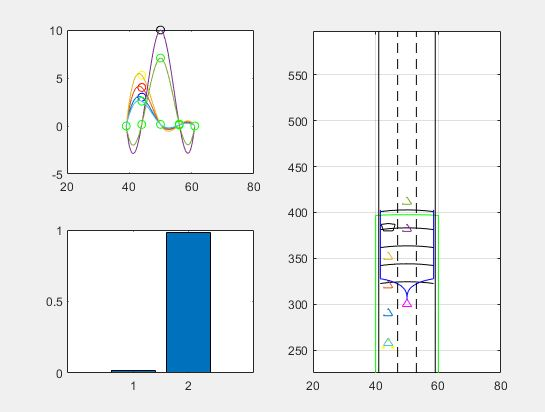
\includegraphics[width=0.5\textwidth]{cs1.JPG}
    \caption{In this snapshot, $u_{\alpha} = 0$ and $u_{h} = 1$. This is because the risk in the vehicle's current lane at $t = t+3$ is well below the $\lambda_{r}$.}
    \label{fig:cs1}
\end{figure}

\begin{figure}[ht]
    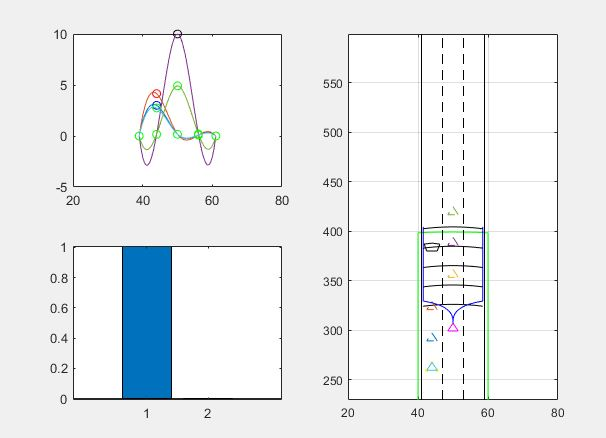
\includegraphics[width=0.5\textwidth]{cs1b.JPG}
    \caption{In this snapshot, the risk in the host vehicle's lane at $t+3$ has increased above $\lambda_{r}$, and autonomy has increased rapidly. The reason $u_{alpha}$ has increased to 1, is because this is the instant at which the change begins. The location of minimum risk is determined to be the right lane, and the vehicle will then move to the right lane.}
    \label{fig:cs1b}
\end{figure}

This simulation results in a safe operation, as the minimum risk is easily identified and the solution is offered. In this simulation, the human takes no action, which is another reason fully autonomous intervention occurs, and the risk is still minimized and avoided.

\subsection{Case Study 2: Dynamic Environment with Lane Change Behavior}
In the second simulation, the human does take some action and it is evident that autonomy and human-control are fluid and change based on changing surroundings. In addition, there is once again a clear location at which the risk is at a minimum. The snapshot in Fig.\ref{fig:cs2} shows a situation where the user is travelling at a velocity slightly too rapid for the obstacle ahead, and slowing down will not put it at a risky position in relation to the next vehicle that is behind the user. As a result, $u_{\alpha}$ is increased as the level of risk increases.
\begin{figure}[ht]
    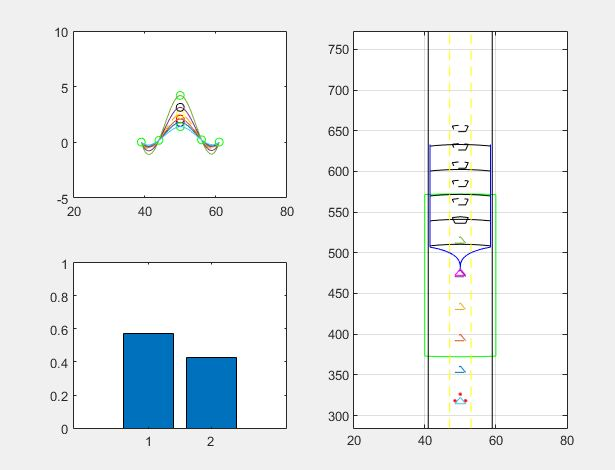
\includegraphics[width=0.5\textwidth]{cs2.JPG}
    \caption{In this snapshot, $u_{\alpha} > u_{h}$. This is because the risk in the vehicle's current lane at $t = t+3$ is slightly above the $\lambda_{r}.$}
    \label{fig:cs2}
\end{figure}
This result also indicates a case of the user's desires being met as closely as possible. The user, by not only adjusting velocity and not adjusting their lane change behavior, indicates that the velocity is the first parameter to adjust. As shown in Fig.\ref{fig:cs2c}, the velocity is only adjusted so that the driver is in a safe position for the selected $t+3$ time and, consequently for times $t+1$ and $t+2$. This is indicated by a velocity that slowly decreases to a safe value. This, however, would only suffice to maximize the time before a collision occurs. Because that is a limitation of only adjusting the velocity, when a collision becomes imminent, $u_\alpha$ increase to 1, and the lane is changed to that of minimum risk.
\begin{figure}[ht]
    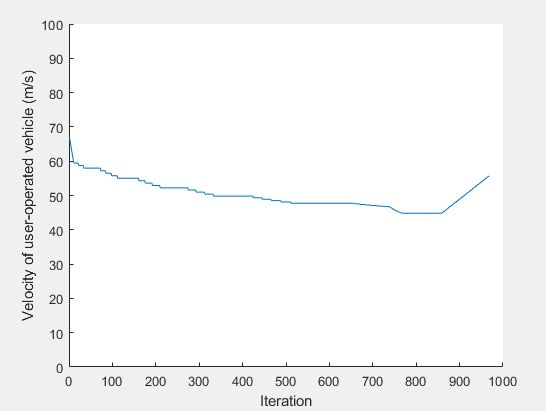
\includegraphics[width=0.5\textwidth]{cs2c.JPG}
    \caption{This figure depicts the velocity of the user's vehicle}
    \label{fig:cs2c}
\end{figure}

\subsection{Case Study 3: Highly dangerous situation with limited options.}
The third case is built much like the second case. In this implementation, however, neither of the two surrounding lanes are available. In this case, the system begins to react much like that of the second case, however, there is a error in the prediction of what the following vehicle will do. This is because the model was trained for a lane change, but it is evident that a lane change will not occur when the actual vehicle (not the estimates) approaches our user's vehicle. An adjustment of the velocities in this case are shown in \ref{fig:vehiclepos}. In a situation like this, the algorithm does delay the imminent collision, but there is a specific preference to retain a certain following distance, $\Delta d$ behind the obstacle in front. We assume that the user's vehicle has a responsibility to not directly cause a collision on its own. This does, however, leave the possibility of a rear collision.




\section{Experiment}
\section{Conclusions}

\newpage
% references section

% can use a bibliography generated by BibTeX as a .bbl file
% BibTeX documentation can be easily obtained at:
% http://mirror.ctan.org/biblio/bibtex/contrib/doc/
% The IEEEtran BibTeX style support page is at:
% http://www.michaelshell.org/tex/ieeetran/bibtex/
%\bibliographystyle{IEEEtran}
% argument is your BibTeX string definitions and bibliography database(s)
%\bibliography{IEEEabrv,../bib/paper}
%
% <OR> manually copy in the resultant .bbl file
% set second argument of \begin to the number of references
% (used to reserve space for the reference number labels box)

%\begin{thebibliography}{1}

%\bibitem{IEEEhowto:kopka}
%H.~Kopka and P.~W. Daly, \emph{A Guide to \LaTeX}, 3rd~ed.\hskip 1em %plus
%  0.5em minus 0.4em\relax Harlow, England: Addison-Wesley, 1999.
  
  
%\end{thebibliography}

%\printbibliography
\bibliographystyle{abbrv}
\bibliography{mybibliography}


% that's all folks
\end{document}


